\documentclass{standalone}
\usepackage{tikz}
\usepackage{ctex,siunitx}
\setCJKmainfont{Noto Serif CJK SC}
\usepackage{tkz-euclide}
\usepackage{amsmath}
\usetikzlibrary{patterns, calc}
\usetikzlibrary {decorations.pathmorphing, decorations.pathreplacing, decorations.shapes,}
\newcommand\dynanometer[3][0]{
  \begin{scope}[#2,rotate=#1,inner sep=0pt]
    \coordinate (A) at (0,2.0);
    \coordinate (B) at (0,2.0+#3*0.2);
    \foreach \x/\y in {100/2.0, 70/1.5, 50/1.2, 30/0.7 }
    {
      \draw[line width=\y pt,gray!\x ]([yshift=1cm]B)circle(0.2);
    }
    \fill[top color=gray, bottom color=gray,middle color=white]([xshift=-1mm,yshift=7mm]B)rectangle([xshift=1mm,yshift=8.7mm]B);
    \fill[green!30!black]([xshift=2.8mm,yshift=6mm]B)--([xshift=2.8mm,yshift=-1.2cm]B)to[bend left=50]([xshift=-2.8mm,yshift=-1.2cm]B)--([xshift=-2.8mm,yshift=6mm]B)to[bend left=50]cycle;
    \fill[lightgray,even odd rule](0.1,0.4)arc(360:180:0.1)--++(0,1.6)--++(0.2,0)--cycle(0,0.4)circle(0.05)([xshift=-0.4mm]A)rectangle++(0.8mm,0.5mm);
    \fill[lightgray!30,even odd rule]([xshift=2.2mm,yshift=5mm]B)--([xshift=2.2mm,yshift=-1.1cm]B)to[bend left]([xshift=-2.2mm,yshift=-1.1cm]B)[rounded corners=2pt]--([xshift=-2.2mm,yshift=5mm]B)[sharp corners]--([xshift=-1mm,yshift=5mm]B)arc(180:0:0.1)[rounded corners=2pt]--cycle[sharp corners]
    ([xshift=-0.4mm,yshift=2mm]B)rectangle([xshift=0.4mm]A);
    \draw[darkgray](0.1,0.1)arc(360:90:0.1)--++(0,0.15);
    \foreach \x in {0,1,...,9}
    {
      \draw[line width=0.1pt,line join=round,lightgray]([yshift=2mm-\x*0.15mm-\x*#3*0.2mm]B)--++(0.3mm,-0.0375mm-#3*0.05mm)--++(-0.6mm,-0.075mm-#3*0.1mm)--++(0.3mm,-0.0375mm-#3*0.05mm);
    }
    \fill[red]([yshift=-0.2mm]A)--([xshift=-1mm]A)--([xshift=1mm]A);
    \foreach \x in {0,1,2,3,4}
    {
      \draw[ultra thin]([xshift=0.5mm,yshift=-\x*2mm]B)--++(0.07,0)node[rotate=#1,right]{\resizebox{!}{0.5mm}{\x}};
      \draw[ultra thin]([xshift=-0.5mm,yshift=-\x*2mm]B)--++(-0.07,0)node[rotate=#1,left]{\resizebox{!}{0.5mm}{\x}};
      \foreach \y in {1,2,3,4,6,7,8,9}
      {
        \draw[ultra thin]([xshift=0.5mm,yshift=-\x*2mm-\y*0.2mm]B)--++(0.05,0);
        \draw[ultra thin]([xshift=-0.5mm,yshift=-\x*2mm-\y*0.2mm]B)--++(-0.05,0);
      }
      \draw[ultra thin]([xshift=0.5mm,yshift=-\x*2mm-1mm]B)--++(0.06,0);
      \draw[ultra thin]([xshift=-0.5mm,yshift=-\x*2mm-1mm]B)--++(-0.06,0);
    }
    \draw[ultra thin]([xshift=0.5mm,yshift=-1cm]B)--++(0.07,0)node[rotate=#1,right]{\resizebox{!}{0.5mm}{5}};
    \draw[ultra thin]([xshift=-0.5mm,yshift=-1cm]B)--++(-0.07,0)node[rotate=#1,left]{\resizebox{!}{0.5mm}{5}};
  \end{scope}
  }
\begin{document}
\small
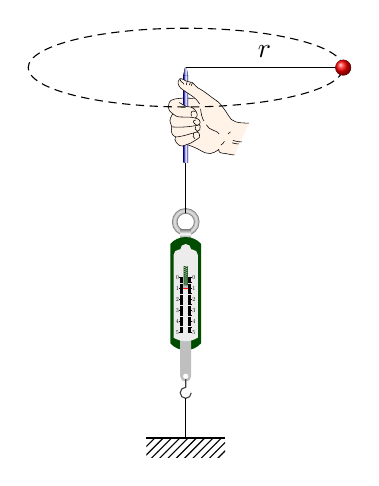
\begin{tikzpicture}[>=latex,scale=1]
  % \useasboundingbox(-1.9,-3.55)rectangle(3,3.15);
  \dynanometer{scale=0.7}{1}
  \draw(0,0)--(0,-0.5)(0,2.35)--(0,3);
  \draw[thick](-0.5,-0.5)--(0.5,-0.5);
  \fill[pattern=north east lines]  (-0.5,-0.5)rectangle(0.5,-0.75);

  \fill[pink!10!orange!10,draw=black,very thin]
  ( 0.802,3.496)..controls( 0.660,3.493)and( 0.580,3.513)..
( 0.548,3.583)..controls( 0.520,3.628)and( 0.448,3.741)..
( 0.401,3.773)..controls( 0.286,3.821)and( 0.213,3.837)..
( 0.134,3.819)..controls( 0.068,3.797)and( 0.014,3.822)..
(-0.074,3.810)..controls(-0.187,3.797)and(-0.213,3.787)..
(-0.219,3.711)..controls(-0.222,3.666)and(-0.203,3.641)..
(-0.163,3.613)..controls(-0.156,3.487)and(-0.081,3.361)..
(-0.012,3.232)..controls( 0.067,3.206)and( 0.130,3.182)..
( 0.183,3.151)..controls( 0.291,3.085)and( 0.340,3.101)..
( 0.421,3.161)..controls( 0.411,3.136)and( 0.424,3.121)..
( 0.466,3.113)..controls( 0.526,3.110)and( 0.576,3.088)..( 0.621,3.092);
  \fill[left color=blue!60!black,right color=blue!60!black,middle color=white](-0.03,3)rectangle(0.03,4.1);
  \fill[left color=blue!60!black,right color=blue!60!black,middle color=white](0.01,4.2)--(0.03,4.1)--(-0.03,4.1)--(-0.01,4.2);
  \fill[pink!10!orange!10,draw=black,very thin]
  ( 0.177,3.737)..controls( 0.126,3.826)and( 0.066,3.845)..
(-0.033,3.916)..controls(-0.130,3.970)and(-0.107,4.095)..
(-0.034,4.051)..controls( 0.025,4.009)and( 0.045,4.029)..
( 0.083,4.011)..controls( 0.102,4.000)and( 0.128,3.958)..
( 0.154,3.942)..controls( 0.246,3.898)and( 0.318,3.826)..( 0.401,3.773)
(-0.085,3.756)..controls(-0.049,3.743)and( 0.011,3.694)..
( 0.035,3.703)..controls( 0.059,3.703)and( 0.071,3.702)..
( 0.111,3.671)..controls( 0.154,3.630)and( 0.160,3.566)..
( 0.117,3.560)..controls( 0.077,3.571)and( 0.040,3.574)..
(-0.007,3.572)..controls(-0.075,3.575)and(-0.107,3.561)..(-0.163,3.613)
(-0.163,3.613)..controls(-0.182,3.589)and(-0.214,3.532)..
(-0.194,3.498)..controls(-0.185,3.478)and(-0.183,3.461)..
(-0.177,3.447)..controls(-0.193,3.385)and(-0.174,3.333)..
(-0.129,3.321)..controls(-0.140,3.300)and(-0.142,3.274)..
(-0.121,3.251)..controls(-0.105,3.231)and(-0.089,3.204)..
(-0.040,3.204)..controls(-0.007,3.205)and(-0.008,3.220)..
( 0.025,3.227)..controls( 0.090,3.244)and( 0.107,3.276)..
( 0.144,3.291)..controls( 0.174,3.306)and( 0.178,3.311)..
( 0.176,3.342)..controls( 0.174,3.366)and( 0.163,3.381)..
( 0.140,3.383)..controls( 0.177,3.393)and( 0.190,3.421)..
( 0.184,3.460)..controls( 0.180,3.470)and( 0.178,3.472)..
( 0.152,3.468)..controls( 0.175,3.476)and( 0.185,3.490)..
( 0.184,3.508)..controls( 0.182,3.528)and( 0.169,3.549)..
( 0.117,3.560)..controls( 0.077,3.571)and( 0.040,3.574)..
(-0.007,3.572)..controls(-0.075,3.575)and(-0.107,3.561)..(-0.163,3.613);
\draw[very thin]
( 0.072,3.581)..controls( 0.060,3.646)and( 0.079,3.660)..( 0.122,3.641)
( 0.129,3.534)..controls( 0.078,3.534)and( 0.094,3.491)..( 0.139,3.470)
( 0.100,3.365)..controls( 0.088,3.332)and( 0.094,3.311)..( 0.117,3.296)
(-0.177,3.447)..controls(-0.054,3.438)and( 0.053,3.448)..( 0.151,3.468)
(-0.129,3.321)..controls(-0.112,3.315)and(-0.037,3.331)..
( 0.027,3.349)..controls( 0.085,3.369)and( 0.115,3.370)..( 0.140,3.383)
( 0.127,3.454)..controls( 0.109,3.425)and( 0.117,3.406)..( 0.149,3.395)
( 0.189,3.677)..controls( 0.195,3.606)and( 0.211,3.550)..( 0.232,3.522)
( 0.262,3.475)..controls( 0.294,3.394)and( 0.399,3.410)..( 0.426,3.358)
( 0.491,3.264)..controls( 0.488,3.240)and( 0.465,3.235)..( 0.446,3.216)
( 0.589,3.245)..controls( 0.620,3.234)and( 0.654,3.229)..( 0.676,3.231)
( 0.599,3.276)..controls( 0.655,3.258)and( 0.685,3.255)..( 0.713,3.257)
( 0.538,3.358)..controls( 0.542,3.371)and( 0.555,3.382)..( 0.568,3.384)
(-0.061,4.052)..controls(-0.091,4.028)and(-0.029,4.015)..(-0.023,3.988)
( 0.016,4.015)..controls( 0.005,4.004)and( 0.007,3.989)..( 0.008,3.979)
( 0.045,3.980)..controls( 0.057,3.987)and( 0.061,3.997)..( 0.061,4.011)
( 0.069,3.970)..controls( 0.081,3.979)and( 0.084,3.990)..( 0.084,4.001);
\draw[densely dashed](0,4.2)ellipse(2 and 0.5);
\draw(0,4.2)--(2,4.2)node[midway,above]{$r$};
\fill[ball color=red](2,4.2)circle(0.1);

\end{tikzpicture}
\end{document}